\subsection{Elenco dei casi d'uso}

%---------------------------- UC1 ---------------------------------
\begin{figure}[H]
    \centering
    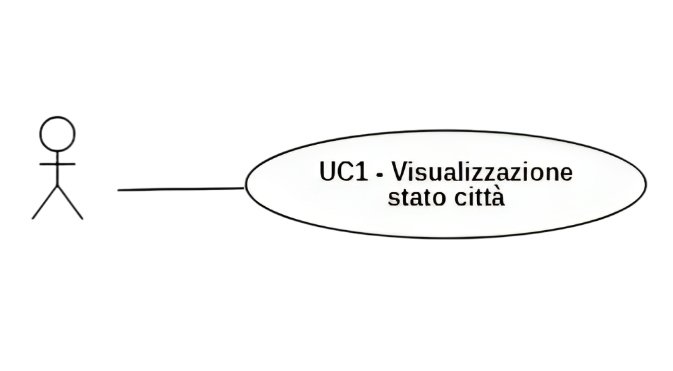
\includegraphics[width=0.9\textwidth]{../Images/uc1.png}
    \caption{UC1 - Visualizzazione stato città}
    \label{fig:UC1}
\end{figure}
\subsubsection{UC1 - VISUALIZZAZIONE DASHBOARD}
\begin{itemize}
    \item \textbf{Attore principale:} Autorità locale.
    \item \textbf{Precondizioni:}
        \begin{itemize}
            \item Il sistema è operativo e accessibile.
        \end{itemize}
    \vspace{0,5cm}
    \item \textbf{Postcondizioni:}
    \begin{itemize}
        \item  L'autorità locale ha una visione aggiornata dello stato di salute della città tramite widget e grafici interattivi aggiornati in tempo reale, una mappa dei sensori presenti nella città e un punteggio di salute relativo alla città.
    \end{itemize}
    \item \textbf{Scenario principale:}
        \begin{enumerate}
            \item L'autorità locale accede alla piattaforma per la visualizzazione della dashboard;
            \item Il sistema elabora le informazioni ricevute dai sensori;
            \item Il sistema imposta la visualizzazione dei widget sulla dashboard.
        \end{enumerate}
    \item \textbf{User story associata:} \\
        Come autorità locale, voglio accedere alla dashboard per visualizzare in tempo reale i dati provenienti dai diversi tipi di sensori presenti nella città. Questo mi consentirà di valutare rapidamente lo stato generale della città e prendere decisioni informate e tempestive sulla gestione delle risorse e sull'implementazione di servizi.
\end{itemize}

%---------------------------- SUB_UC1 ---------------------------------
\begin{figure}[H]
    \centering
    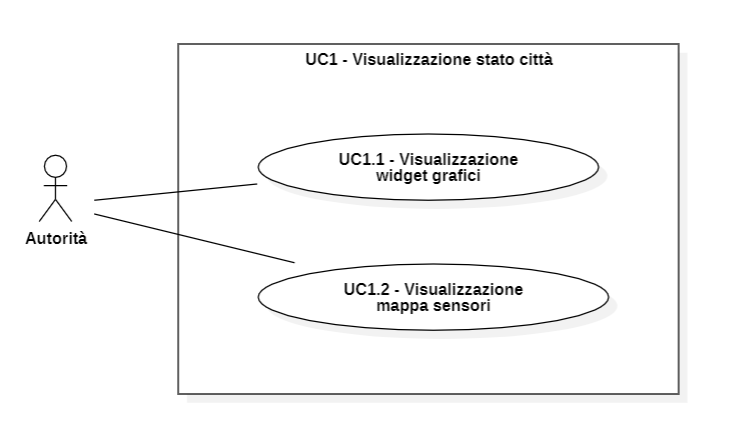
\includegraphics[width=0.9\textwidth]{../Images/uc1_Subcase.PNG} 
    \caption{Sottocasi UC1 - Visualizzazione stato città}
    \label{fig:UC1_sub}
\end{figure}

%---------------------------- UC1.1 ---------------------------------
\subsubsection{UC1.1 - PANORAMICA COMPLESSIVA DEI WIDGET DI MISURAZIONE PER OGNI TIPOLOGIA DI SENSORE}
\begin{itemize}
    \item \textbf{Attore principale:} Autorità locale.
    \item \textbf{Descrizione:} L'autorità locale accede alla dashboard della città e visualizza un widget contente un grafico aggiornato in tempo reale, il quale rappresenta i dati registrati durante la giornata per ogni tipologia di sensore che trasmette al sistema.
    \item \textbf{Scenario principale:}
        \begin{enumerate}
            \item L'utente accede alla piattaforma per la visualizzazione della dashboard della città. (UC1)
            \item Il sistema elabora le informazioni ricevute dai sensori e imposta la visualizzazione di un widget con le misurazioni quotidiane per ogni tipolgia di sensore;
        \end{enumerate}
    \item \textbf{Precondizioni:}
        \begin{itemize}
            \item Nessuna
        \end{itemize}
    \item \textbf{Postcondizioni:}
        \begin{itemize}
            \item L'autorità locale ha una visione di un widget con misurazioni aggiornate in tempo reale, il quale rappresenta i dati registrati durante la giornata per ogni tipologia di sensore.
        \end{itemize}
    \item \textbf{User story associata:}
        \begin{itemize}
            \item Come autorità locale voglio visualizzare widget come le misurazioni aggiornate in tempo reale sui dati registrati durante la giornata per ogni tipologia di sensore nella dashboard.
        \end{itemize}
\end{itemize}


%---------------------------- UC1.2 ---------------------------------
\subsubsection{UC1.2 - Visualizzazione mappa sensori}
\begin{itemize}
    \item \textbf{Attore principale:} Autorità locale.
    \item \textbf{Descrizione:} L'autorità locale accede alla dashboard della città e visualizza una mappa con una visione dei sensori posizionati nella città.
    \item \textbf{Scenario principale:}
          \begin{enumerate}
              \item L'utente visualizza una mappa contenente i sensori nella corretta posizione. (i sensori sono etichettati per riconoscere la tipologia)
          \end{enumerate}
    \item \textbf{Precondizioni:}
          \begin{itemize}
              \item  Almeno un sensore è attivo e ha trasmesso dati;
              \item L'utente si trova nella dashboard della città. (UC1)
          \end{itemize}
    \item \textbf{Postcondizioni:}
          \begin{itemize}
              \item      L'utente ha una visione grafica aggiornata della mappa dei sensori nella città e della loro tipologia.
          \end{itemize}
    \item \textbf{User story associata:}
          \begin{itemize}
              \item Come autorità locale, voglio essere in grado di visualizzare una mappa contenente i sensori attivi e operativi all'interno della città. La mappa deve mostrare chiaramente la posizione di ciascun sensore e devono essere etichettati per consentire un riconoscimento immediato della tipologia di ogni sensore.
          \end{itemize}
\end{itemize}

%---------------------------- UC1.3 ---------------------------------
\subsubsection{UC1.3 - VISUALIZZAZIONE WIDGET PUNTEGGIO DI SALUTE}
\begin{itemize}
    \item \textbf{Attore principale:} Autorità locale.
    \item \textbf{Precondizioni:}
        \begin{itemize}
            \item Il sistema è operativo e accessibile.
        \end{itemize}
    \item \textbf{Postcondizioni:}
        \begin{itemize}
            \item L'autorità locale ha una visione aggiornata di un punteggio, un numero intero, rappresentante lo stato di salute della città.
        \end{itemize}
    \item \textbf{Scenario principale:}
          \begin{enumerate}
            \item L'autorità locale accede alla piattaforma per la visualizzazione della dashboard. (UC1)
            \item Il sistema elabora i dati provenienti dai sensori e calcola un punteggio di salute.
        \end{enumerate}
    \item \textbf{User story associata:} \\
        Come autorità locale, desidero visualizzare un punteggio ottenuto tramite una funzione di aggregazione, il quale fornisca una visione immediata di eventuali dati anomali rilevati dai sensori disseminati nella città, al fine di identificare rapidamente situazioni critiche e prendere azioni tempestive per garantire la sicurezza e il benessere della comunità.
\end{itemize}

%---------------------------- UC2 ---------------------------------
\begin{figure}[H]
    \centering
    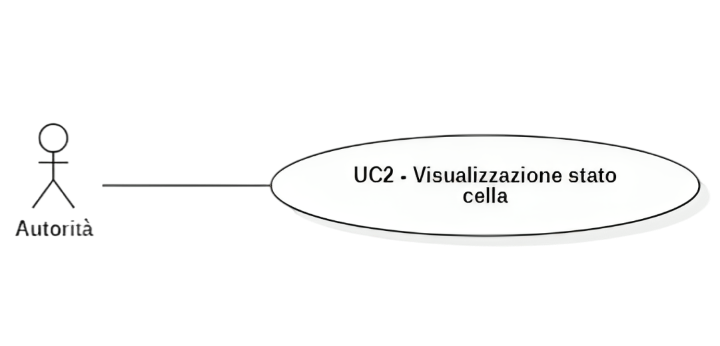
\includegraphics[width=0.9\textwidth]{../Images/uc2.png}
    \caption{UC2 - Visualizzazione stato cella}
    \label{fig:UC2}
\end{figure}
\subsubsection{UC2 - Visualizzazione stato cella}
\begin{itemize}
    \item \textbf{Attore principale:} Autorità locale.
    \item \textbf{Descrizione:} L'autorità locale effettua la selezione della cella, ossia la specifica zona urbana, al fine di visualizzare in tempo reale i dati provenienti da varie tipologie di sensori ubicati nella suddetta area. Ciò permette una valutazione reapida dello stato complessivo della cella.
    \item \textbf{Scenario principale:}
        \begin{enumerate}
            \item L'utente seleziona la cella per la quale desidera visualizzare la dashboard contenente esclusivamente i dati correlati a essa.
        \end{enumerate}
    \item \textbf{Precondizioni:}
        \begin{itemize}
            \item  Almeno un sensore presente nella cella ha trasmesso dati;
            \item L'utente si trova  nella piattaforma per la visualizzazione della dashboard sullo stato della città (UC1);
        \end{itemize}
    \item \textbf{Postcondizioni:}
        \begin{itemize}
            \item  L'utente ha una visione aggiornata dello stato di salute della cella tramite widget e grafici interattivi aggiornati in tempo reale sulla base di dati correlati esclusivamente alla cella, inoltre visualizza una mappa dei sensori presenti nella cella e un punteggio di salute relativo alla cella.
          \end{itemize}
    \item \textbf{User story associata:}
        \begin{itemize}
            \item Come autorità locale, desidero poter selezionare una specifica cella urbana sulla piattaforma al fine di visualizzare immediatamente i dati provenienti da vari sensori presenti nell'area. Questo mi permetterà di valutare rapidamente lo stato complessivo della cella e prendere decisioni informate.
        \end{itemize}
\end{itemize}

%---------------------------- UC3 ---------------------------------
\begin{figure}[H]
    \centering
    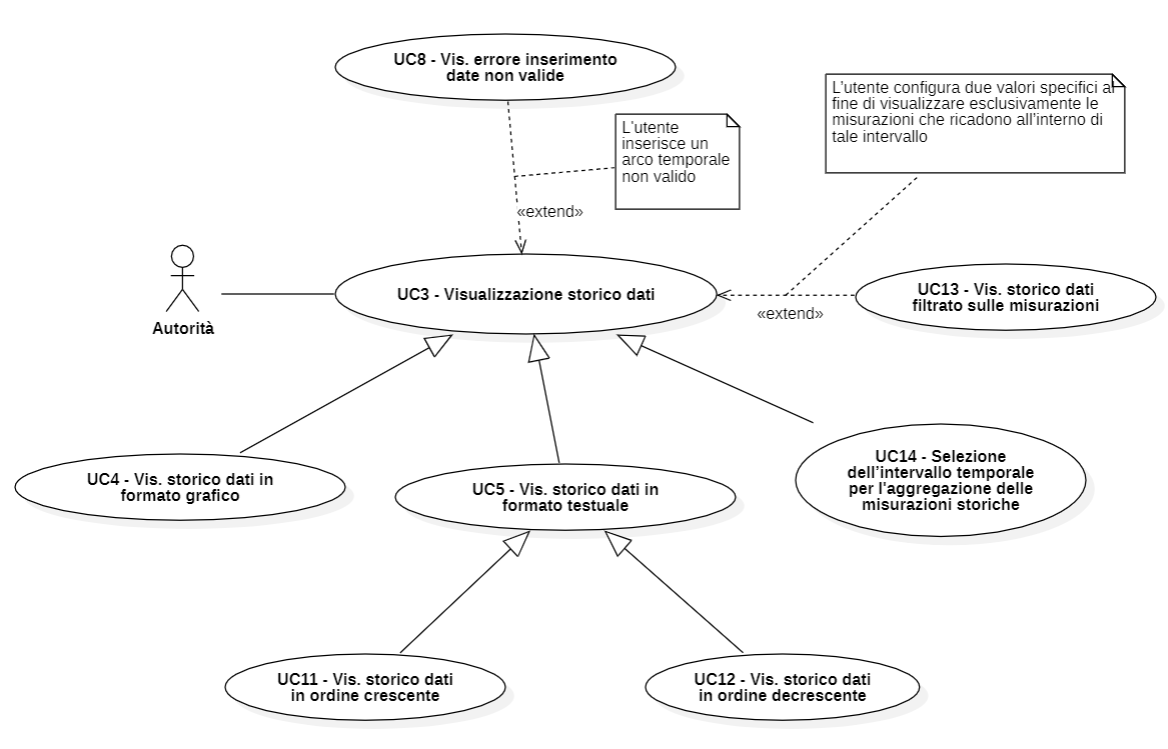
\includegraphics[width=0.9\textwidth]{../Images/uc3.png}
    \caption{UC3 - Visualizzazione storico dati }
    \label{fig:UC3}
\end{figure}
\subsubsection{UC3 - VISUALIZZAZIONE WIDGET MISURAZIONI DI UNA TIPOLOGIA SPECIFICA DI SENSORI}

\begin{itemize}
    \item \textbf{Attore principale:} Autorità locale;
    \item \textbf{Precondizioni:}
        \begin{itemize}
            \item Almeno un sensore della tipologia associata al widget ha trasmesso dati al sistema.
            \item Il sistema ha caricato la visualizzazione della dashboard (UC1);
        \end{itemize}
    \item \textbf{Postcondizioni:}
        \begin{itemize}
            \item L'autorità locale visualizza uno specifico widget contenente le misurazioni rilevate da una specifica tipologia di sensori.
        \end{itemize}
    \item \textbf{Scenario principale:}
        \begin{enumerate}
            \item Il sistema carica i dati e imposta la visualizzazione di uno specifico widget contenente le misurazioni relative ad una specifica tipologia di sensori.
        \end{enumerate}
    \item \textbf{User story associata:} \\
        Come autorità locale, voglio accedere a un widget dettagliato che rappresenti le misurazioni provenienti da una specifica tipologia di sensori. Questo mi permetterà di analizzare in modo approfondito i dati relativi a quella tipologia di sensori, aiutandomi a prendere decisioni mirate per migliorare i servizi della città.
\end{itemize}

%---------------------------- SUB_UC3 ---------------------------------
\begin{figure}[H]
    \centering
    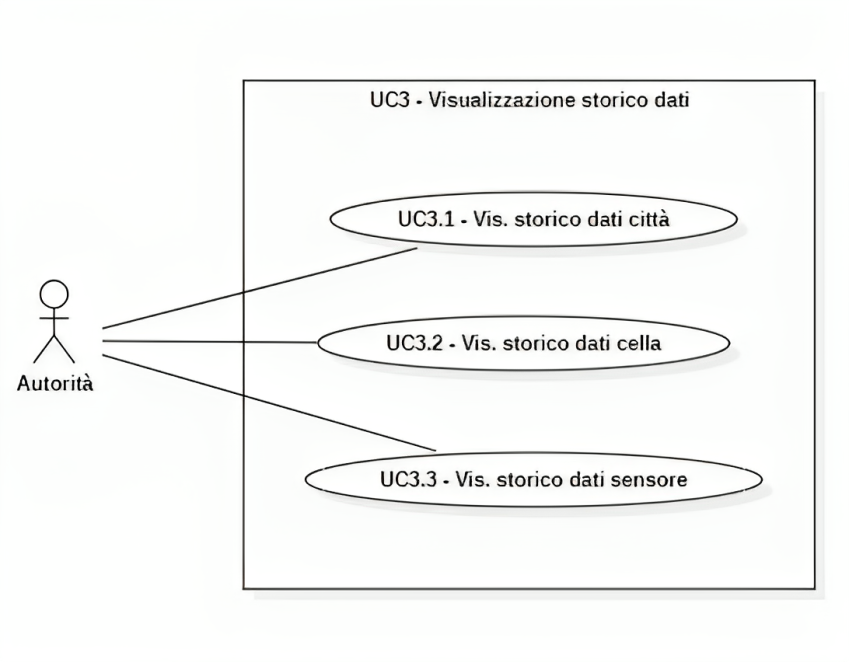
\includegraphics[width=0.9\textwidth]{../Images/uc3_Subcase.png}
    \caption{Sottocasi UC3 - Visualizzazione storico dati }
    \label{fig:UC3_sub}
\end{figure}

%---------------------------- UC3.1 ---------------------------------
\subsubsection{UC3.1 - VISUALIZZAZIONE INFORMAZIONI SENSORI}
\begin{itemize}
    \item \textbf{Attore principale:} Autorità locale;
    %\item \textbf{Descrizione:} L'autorità locale procede all'accesso alla piattaforma e, mediante la dashboard relativa allo stato di salute della città, effettua la selezione di una specifica categoria di sensori al fine di visualizzare esclusivamente i dati storici ad essi pertinenti.
    \item \textbf{Scenario principale:}
        \begin{enumerate}
            \item Il sistema carica e imposta la visualizzazione delle informazioni dei sensori coinvolti.
        \end{enumerate}
    \item \textbf{Precondizioni:}
        \begin{itemize}
            \item Il sistema ha caricato e impostato la visualizzazione di un widget di una specifica tipolgia di sensori (UC3);
            \item Almeno un sensore contribuisce alle misurazioni rappresentate nel widget.
        \end{itemize}
    \item \textbf{Postcondizioni:}
        \begin{itemize}
            \item  L'autorità locale ha una visione sugli identificativi dei sensori che contribuiscono alle misurazioni reappresentate nel widget.
        \end{itemize}
    \item \textbf{User story associata:}
        \begin{itemize}
            \item Come Autorità Locale, desidero visualizzare informazioni quali l'identificativo dei sensori coinvolti nel widget di misurazioni.
        \end{itemize}
\end{itemize}

%---------------------------- UC3.2 ---------------------------------
\subsubsection{UC3.2 - VISUALIZZAZIONE MISURAZIONI SENSORI NEL TEMPO}
\begin{itemize}
    \item \textbf{Attore principale:} Autorità locale;
    %\item \textbf{Descrizione:} L'autorità locale procede all'accesso alla piattaforma e, mediante la dashboard relativa allo stato di salute della città, effettua la selezione di una specifica categoria di sensori al fine di visualizzare esclusivamente i dati storici ad essi pertinenti.
    \item \textbf{Scenario principale:}
        \begin{enumerate}
            \item Il sistema carica e imposta la visualizzazione delle misurazioni dei sensori coinvolti.
        \end{enumerate}
    \item \textbf{Precondizioni:}
        \begin{itemize}
            \item Il sistema ha caricato e impostato la visualizzazione di un widget di una specifica tipolgia di sensori (UC3);
            \item Almeno un sensore contribuisce alle misurazioni rappresentate nel widget.
        \end{itemize}
    \item \textbf{Postcondizioni:}
        \begin{itemize}
            \item  L'autorità locale visualizza le misurazioni dei sensori che contribuiscono al widget.
        \end{itemize}
    \item \textbf{User story associata:}
        \begin{itemize}
            \item Come Autorità Locale, desidero visualizzare le misurazioni dei sensori di una specifica categoria per poter effettuare analisi mirate.
        \end{itemize}
\end{itemize}

\begin{figure}[H]
    \centering
    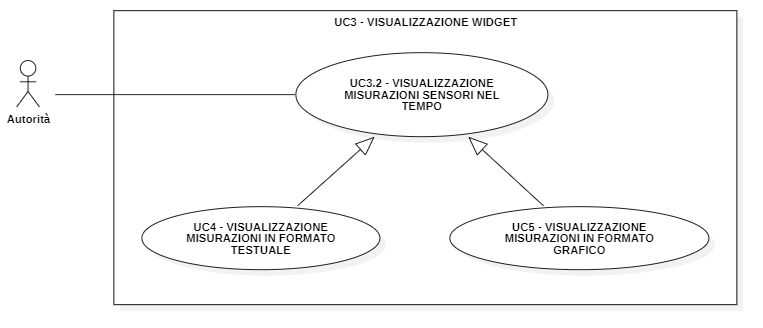
\includegraphics[width=0.9\textwidth]{../Images/uc3_1Gen.PNG.png}
    \caption{UC3.2 - Visualizzazione storico dati }
    \label{fig:UC3_gen}
\end{figure}

%---------------------------- UC3.1 ---------------------------------
\subsubsection{UC4 - Visualizzazione storico dati in formato testuale}
\begin{itemize}
    \item \textbf{Attore principale:} Autorità locale;
    \item \textbf{Descrizione:} L’autorità locale seleziona i/il sensore/i della quale vuole visionare lo storico dei dati e imposta la visulizzazione in formato testuale: (TIMESTAMP, Dato).
    \item \textbf{Scenario principale:}
          \begin{enumerate}
              \item L'utente imposta la visualizzazione in formato testuale.
          \end{enumerate}
    \item \textbf{Precondizioni:}
          \begin{itemize}
              \item  I/Il sensori/e di cui si vogliono visualizzare i dati storici ha trasmesso dati;
              \item  L'utente si trova in un interfaccia per la visualizzazione di uno storico dati (UC3).
          \end{itemize}
    \item \textbf{Postcondizioni:}
          \begin{itemize}
              \item  L'utente ha una visione dello storico dei dati trasmessi nel formato (TIMESTAMP, dato).
          \end{itemize}
    \item \textbf{User story associata:}
          \begin{itemize}
              \item Come autorità locale,
                    desidero visualizzare lo storico dei dati in formato testuale (TIMESTAMP, Dato),
                    In modo da avere una visione dettagliata delle informazioni trasmesse dai sensori.
          \end{itemize}
\end{itemize}

%---------------------------- UC3.2 ---------------------------------
\subsubsection{UC5 - VISUALIZZAZIONE MISURAZIONI IN FORMATO GRAFICO \newline TIME SERIES}
\begin{itemize}
    \item \textbf{Attore principale:} Autorità locale;
    \item \textbf{Precondizioni:}
        \begin{itemize}
            \item Il sistema è operativo e accessibile.
        \end{itemize}
    \item \textbf{Postcondizioni:}
        \begin{itemize}
            \item L'utente visualizza le misurazioni associate al widget attraverso un grafico time series.
        \end{itemize}
    \vspace{1cm}
    \item \textbf{Scenario principale:}
        \begin{enumerate}
            \item Il sistema carica e configura la visualizzazione di un widget di una specifica tipologia di sensori (UC1.1.1);
                \item Il sistema carica e configura la visualizzazione all'interno del widget delle misurazioni dei sensori coinvolti;
                \item L'autorità locale seleziona la visualizzazione delle misurazioni associato al widget in formato grafico.
        \end{enumerate}
    \item \textbf{User story associata:} \\
        Come autorità locale, desidero visualizzare le misurazioni associate ad uno specifico widget attraverso un grafico time series. Questo consente di semplificare la comprensione e la comparazione delle misurazioni, permettendo di individuare tendenze, relazioni e pattern in modo chiaro e rapido.
\end{itemize}


%---------------------------- UC6 ---------------------------------
\begin{figure}[H]
    \centering
    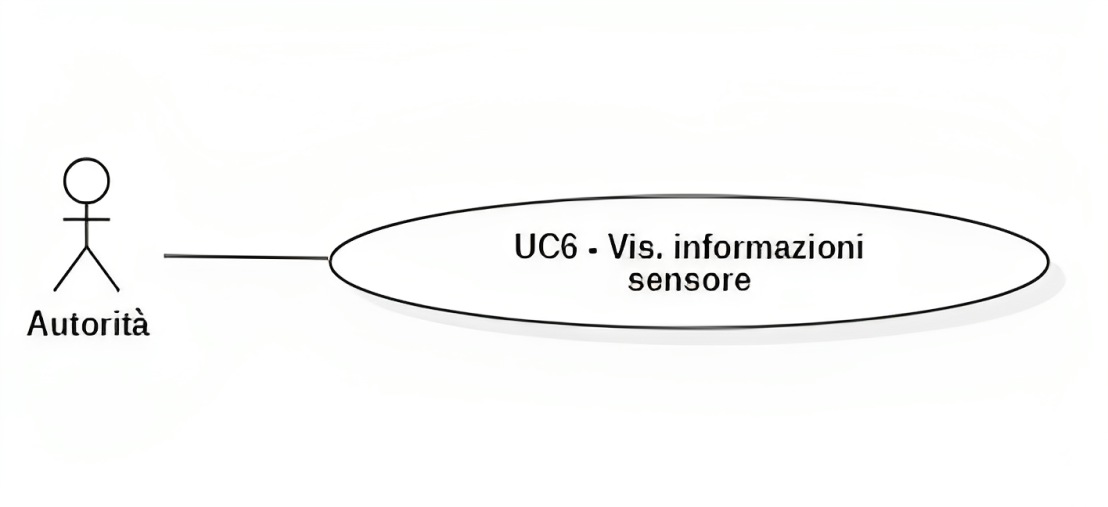
\includegraphics[width=0.9\textwidth]{../Images/uc6.png}
    \caption{UC6 - Visualizzazione informazioni sensore}
    \label{fig:UC6}
\end{figure}
\subsubsection{UC6 - VISUALIZZAZIONE WIDGET SENSORI TEMPERATURA}
\begin{itemize}
    \item \textbf{Attore principale:} Autorità locale;
    \item \textbf{Precondizioni:}
        \begin{itemize}
            \item Almeno un sensore di temperatura ha trasmesso dati al sistema;
            \item Il sistema ha caricato la visualizzazione della dashboard (UC1).
        \end{itemize}
    \item \textbf{Postcondizioni:}
        \begin{itemize}
            \item L'autorità locale visualizza un widget contenente le misurazioni relative ai sensori di temperatura.
        \end{itemize}
    \item \textbf{Scenario principale:}
        \begin{enumerate}
            \item Il sistema carica i dati e imposta la visualizzazione del widget contenente le misurazioni relative ai sensori di temperatura.
        \end{enumerate}
    \item \textbf{User story associata:} \\
        Come autorità locale, desidero visualizzare un widget per la visualizzazione delle misurazioni trasmesse dai sensori di temperatura. Questo mi permetterà di analizzare in modo approfondito i dati relativi a quella tipologia di sensori, aiutandomi a prendere decisioni mirate per migliorare i servizi della città.
\end{itemize}

%---------------------------- SUB_UC6 ---------------------------------
\begin{figure}[H]
    \centering
    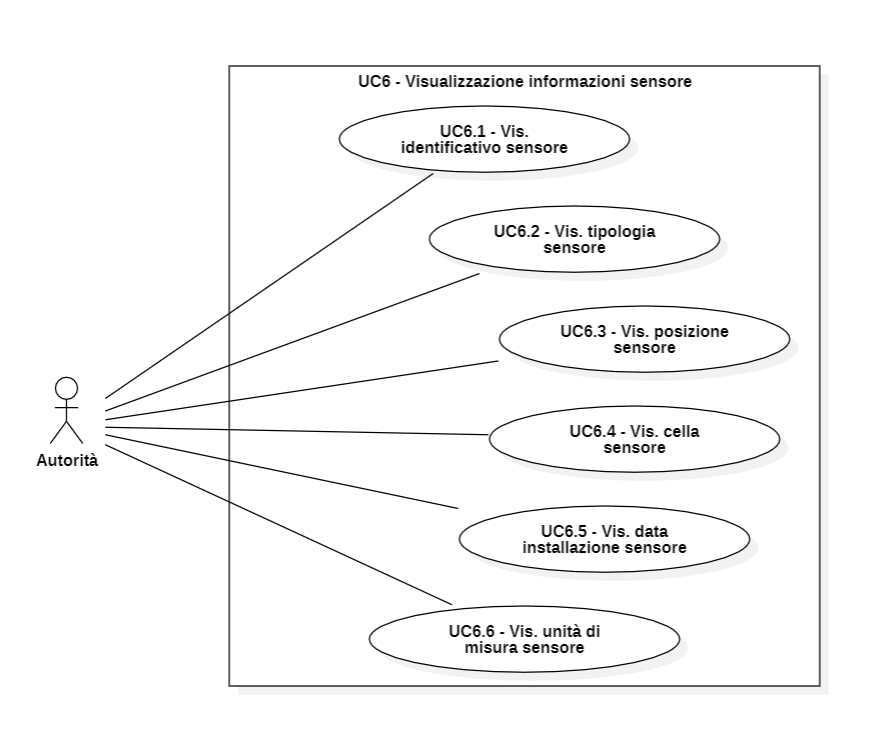
\includegraphics[width=0.9\textwidth]{../Images/uc6_Subcase.PNG}
    \caption{Sottocasi UC6 - Visualizzazione informazioni sensore}
    \label{fig:UC6_sub}
\end{figure}

%---------------------------- UC6.1 ---------------------------------
\subsubsection{UC6.1 - Visualizzazione Identificativo sensore}
\begin{itemize}
    \item \textbf{Attore principale:} Autorità locale;
    \item \textbf{Descrizione:} L’autorità locale dalla pagina adibita alla visione delle informazioni di un sensore visualizza il suo Identificativo.
    \item \textbf{Scenario principale:}
          \begin{enumerate}
              \item L'utente visualizza l'Identificativo del sensore.
          \end{enumerate}
    \item \textbf{Precondizioni:}
          \begin{itemize}
              \item  L'utente di trova nella pagina di visualizzazione delle informazioni di un sensore (UC6.1)
          \end{itemize}
    \item \textbf{Postcondizioni:}
          \begin{itemize}
              \item  L'utente visualizza l'Identificativo del sensore.
          \end{itemize}\item \textbf{User story associata:}
          \begin{itemize}
              \item Come Autorità Locale, desidero visualizzare l'identificativo di un sensore dalla pagina dedicata alle informazioni del sensore.
          \end{itemize}
\end{itemize}

%---------------------------- UC6.2 ---------------------------------
\subsubsection{UC6.2 - Visualizzazione tipologia sensore}
\begin{itemize}
    \item \textbf{Attore principale:} Autorità locale;
    \item \textbf{Descrizione:} L’autorità locale dalla pagina adibita alla visione delle informazioni di un sensore visualizza la sua tipologia (ex. Termometro).
    \item \textbf{Scenario principale:}
    \begin{enumerate}
        \item L'utente seleziona la visualizzazione delle informazioni del sensore.
    \end{enumerate}
\item \textbf{Precondizioni:}
    \begin{itemize}
        \item  L'utente di trova nella pagina di visualizzazione dello storico dei dati di un sensore. (3.3)
    \end{itemize}
    \item \textbf{Postcondizioni:}
          \begin{itemize}
              \item  L'utente visualizza la tipologia del sensore.
          \end{itemize}\item \textbf{User story associata:}
          \begin{itemize}
              \item Come Autorità Locale, desidero visualizzare la tipolgia di un sensore dalla pagina dedicata alle informazioni del sensore.
          \end{itemize}
\end{itemize}

%---------------------------- UC6.3 ---------------------------------
\subsubsection{UC6.3 - Visualizzazione posizione sensore}
\begin{itemize}
    \item \textbf{Attore principale:} Autorità locale;
    \item \textbf{Descrizione:} L’autorità locale dalla pagina adibita alla visione delle informazioni di un sensore visualizza la sua posizione in coordinate.
    \item \textbf{Scenario principale:}
          \begin{enumerate}
              \item L'utente visualizza le coordinate del sensore.
          \end{enumerate}
    \item \textbf{Precondizioni:}
          \begin{itemize}
              \item  L'utente di trova nella pagina di visualizzazione delle informazioni di un sensore (UC6.1)
          \end{itemize}
    \item \textbf{Postcondizioni:}
          \begin{itemize}
              \item  L'utente visualizza le coordinate del sensore.
          \end{itemize}
    \item \textbf{User story associata:}
          \begin{itemize}
              \item Come Autorità Locale, desidero visualizzare la posizione di un sensore, in coordinate, dalla pagina dedicata alle informazioni del sensore.
          \end{itemize}
\end{itemize}

%---------------------------- UC6.4 ---------------------------------
\subsubsection{UC6.4 - Visualizzazione cella sensore}
\begin{itemize}
    \item \textbf{Attore principale:} Autorità locale;
    \item \textbf{Descrizione:} L’autorità locale dalla pagina adibita alla visione delle informazioni di un sensore visualizza la cella dove è installato il sensore.
    \item \textbf{Scenario principale:}
    \begin{enumerate}
        \item L'utente seleziona la visualizzazione dell'informazioni del sensore.
    \end{enumerate}
\item \textbf{Precondizioni:}
    \begin{itemize}
        \item  L'utente di trova nella pagina di visualizzazione dello storico dei dati di un sensore. (3.3)
    \end{itemize}
    \item \textbf{Postcondizioni:}
          \begin{itemize}
              \item  L'utente visualizza la cella dove è installato il sensore
          \end{itemize}
    \item \textbf{User story associata:}
          \begin{itemize}
              \item Come Autorità Locale, desidero visualizzare la cella di appartenenza di un sensore dalla pagina dedicata alle informazioni del sensore.
          \end{itemize}
\end{itemize}

%---------------------------- UC6.5 ---------------------------------
\subsubsection{UC6.5 - Visualizzazione data installazione sensore}
\begin{itemize}
    \item \textbf{Attore principale:} Autorità locale;
    \item \textbf{Descrizione:} L’autorità locale dalla pagina adibita alla visione delle informazioni di un sensore visualizza la data di installazione del sensore.
    \item \textbf{Scenario principale:}
    \begin{enumerate}
        \item L'utente seleziona la visualizzazione delle informazioni del sensore.
    \end{enumerate}
\item \textbf{Precondizioni:}
    \begin{itemize}
        \item  L'utente di trova nella pagina di visualizzazione dello storico dei dati di un sensore. (3.3)
    \end{itemize}
    \item \textbf{Postcondizioni:}
          \begin{itemize}
              \item  L'utente visualizza la data di installazione del sensore.
          \end{itemize}
    \item \textbf{User story associata:}
          \begin{itemize}
              \item Come Autorità Locale, desidero visualizzare la data di installazione di un sensore dalla pagina dedicata alle informazioni del sensore.
          \end{itemize}
\end{itemize}

%---------------------------- UC6.6 ---------------------------------
\subsubsection{UC6.6 - Visualizzazione unità misura sensore}
\begin{itemize}
    \item \textbf{Attore principale:} Autorità locale;
    \item \textbf{Descrizione:} L’autorità locale dalla pagina adibita alla visione delle informazioni di un sensore visualizza l'unità di misura del sensore.
    \item \textbf{Scenario principale:}
    \begin{enumerate}
        \item L'utente seleziona la visualizzazione delle informazioni del sensore.
    \end{enumerate}
\item \textbf{Precondizioni:}
    \begin{itemize}
        \item  L'utente di trova nella pagina di visualizzazione dello storico dei dati di un sensore. (3.3)
    \end{itemize}
    \item \textbf{Postcondizioni:}
          \begin{itemize}
              \item  L'utente visualizza l'unità di misura del sensore.
          \end{itemize}
    \item \textbf{User story associata:}
          \begin{itemize}
              \item Come Autorità Locale, desidero visualizzare l'unità di misura di un sensore dalla pagina dedicata alle informazioni del sensore.
          \end{itemize}
\end{itemize}

%---------------------------- UC7 ---------------------------------
\begin{figure}[H]
    \centering
    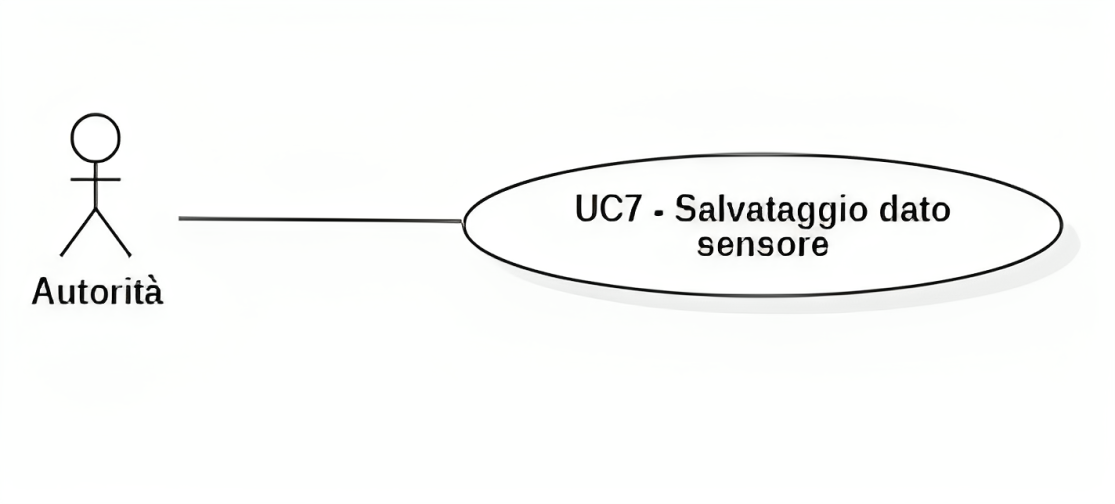
\includegraphics[width=0.9\textwidth]{../Images/uc7.png}
    \caption{UC7 - Salvataggio dato sensore}
    \label{fig:UC7}
\end{figure}
\subsubsection{UC7 - VISUALIZZAZIONE WIDGET SENSORI UMIDITÀ}
\begin{itemize}
    \item \textbf{Attore principale:} Autorità locale;
    \item \textbf{Precondizioni:}
        \begin{itemize}
            \item Il sistema ha caricato la visualizzazione della dashboard (UC1).
        \end{itemize}
    \item \textbf{Postcondizioni:}
        \begin{itemize}
            \item L'autorità locale visualizza un widget contenente le misurazioni relative ai sensori di umidità.
        \end{itemize}
    \item \textbf{Scenario principale:}
        \begin{enumerate}
            \item Il sistema carica i dati e imposta la visualizzazione del widget contenente le misurazioni relative ai sensori di umidità.
        \end{enumerate}
    \item \textbf{User story associata:} \\
        Come autorità locale, desidero visualizzare un widget per la visualizzazione delle misurazioni trasmesse dai sensori di umidità. Questo mi permetterà di analizzare in modo approfondito i dati relativi a quella tipologia di sensori, aiutandomi a prendere decisioni mirate per migliorare i servizi della città.
\end{itemize}

%---------------------------- SUB_UC7 ---------------------------------
\begin{figure}[H]
    \centering
    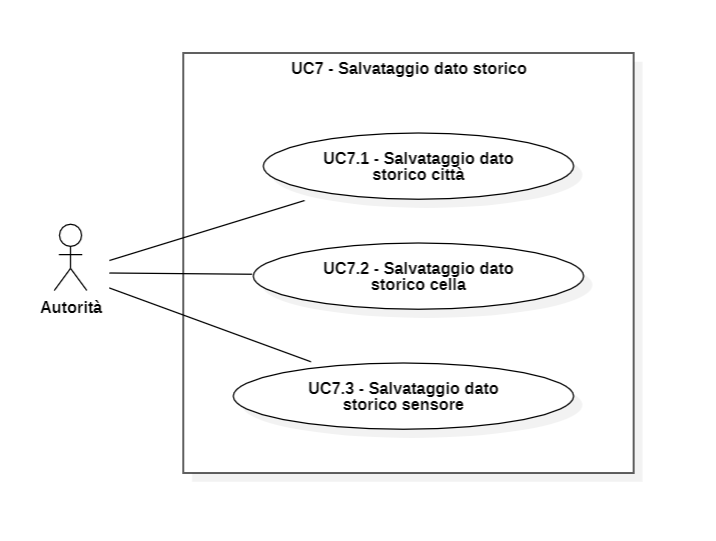
\includegraphics[width=0.9\textwidth]{../Images/uc7_Subcase.PNG}
    \caption{Sottocasi UC7 - Salvataggio dato sensore}
    \label{fig:UC7_sub}
\end{figure}

%---------------------------- UC7.1 ---------------------------------
\subsubsection{UC7.1 - Salvataggio dato storico citta}
\begin{itemize}
    \item \textbf{Attore principale:} Autorità locale;
    \item \textbf{Descrizione:} L’autorità locale dalla pagina adibita alla visulizzazione dello storico dati in formato testuale salva un dato emesso tra i preferiti.
    \item \textbf{Scenario principale:}
          \begin{enumerate}
              \item L'utente salva tra i preferiti uno dei dati storici della città emesso.
          \end{enumerate}
    \item \textbf{Precondizioni:}
          \begin{itemize}
              \item  L'utente si trova nella pagina di visualizzazione  dei dati storici emessi nella città per una tipologia di sensore (UC3.3);
              \item La visualizzazione è impostata nel formato testuale (UC4);
              \item  Il dato che intende salvare tra i preferiti non lo era già in precedenza.
          \end{itemize}
    \item \textbf{Postcondizioni:}
          \begin{itemize}
              \item  Il dato storico della città viene memorizzato nella lista dei preferiti nel
                    formato testuale: (TipoSensore,
                    TIMESTAMP, Dato).
          \end{itemize}
    \item \textbf{User story associata:}
          \begin{itemize}
              \item Come Autorità locale
                    Voglio poter salvare uno dei dati storici emessi dalla città tra i preferiti
                    In modo che possa accedere rapidamente ai dati rilevanti in futuro.
          \end{itemize}
\end{itemize}

%---------------------------- UC7.2 ---------------------------------
\subsubsection{UC7.2 - Salvataggio dato storico cella}
\begin{itemize}
    \item \textbf{Attore principale:} Autorità locale;
    \item \textbf{Descrizione:} L’autorità locale dalla pagina adibita alla visulizzazione dello storico dati in formato testuale relativo ad una cella salva un dato emesso tra i preferiti.
    \item \textbf{Scenario principale:}
          \begin{enumerate}
              \item L'utente seleziona il salvataggio tra i preferiti uno dei dati storici della cella emesso .
          \end{enumerate}
    \item \textbf{Precondizioni:}
          \begin{itemize}
              \item  L'utente si trova nella pagina di visualizzazione dei dati storici emessi in una cella per una tipologia di sensore (UC3.2);
              \item La visualizzazione è impostata nel formato testuale (UC4);
              \item  Il dato che intende salvare tra i preferiti non lo era già in precedenza.
          \end{itemize}
    \item \textbf{Postcondizioni:}
          \begin{itemize}
              \item  Il dato storico della città viene memorizzato nella lista dei preferiti formato testuale (Cella,
                    TipoSensore, TIMESTAMP,
                    Dato)
          \end{itemize}
    \item \textbf{User story associata:}
          \begin{itemize}
              \item Come Autorità locale
                    Voglio poter salvare uno dei dati storici emessi da una cella tra i preferiti
                    In modo che possa accedere rapidamente ai dati rilevanti in futuro.
          \end{itemize}
\end{itemize}


%---------------------------- UC7.3 ---------------------------------
\subsubsection{UC7.3 - Salvataggio dato storico sensore}
\begin{itemize}
    \item \textbf{Attore principale:} Autorità locale;
    \item \textbf{Descrizione:} L’autorità locale dalla pagina adibita alla visulizzazione dei dati emessi da un sensore salva il dato tra i preferiti.
    \item \textbf{Scenario principale:}
          \begin{enumerate}
              \item L'utente salva tra i preferiti uno dei dati storici emessi dal sensore.
          \end{enumerate}
    \item \textbf{Precondizioni:}
          \begin{itemize}
              \item  L'utente si trova nella pagina di visulizzazione in formato testuale dei dati storici emessi da un sensore (UC3.3);
              \item  Il dato che intende salvare tra i preferiti non lo era già in precedenza.
          \end{itemize}
    \item \textbf{Postcondizioni:}
          \begin{itemize}
              \item  Il dato storico emesso dal sensore viene memorizzato nella lista dei preferiti nel formato testuale: (IDSensore,Cella, TipoSensore,
                    TIMESTAMP, Dato).
          \end{itemize}
    \item \textbf{User story associata:}
          \begin{itemize}
              \item Come Autorità locale voglio poter salvare uno dei dati storici emessi da un sensore tra i preferiti in modo che possa accedere rapidamente ai dati rilevanti in futuro.
          \end{itemize}
\end{itemize}


%---------------------------- UC9 ---------------------------------
\begin{figure}[H]
    \centering
    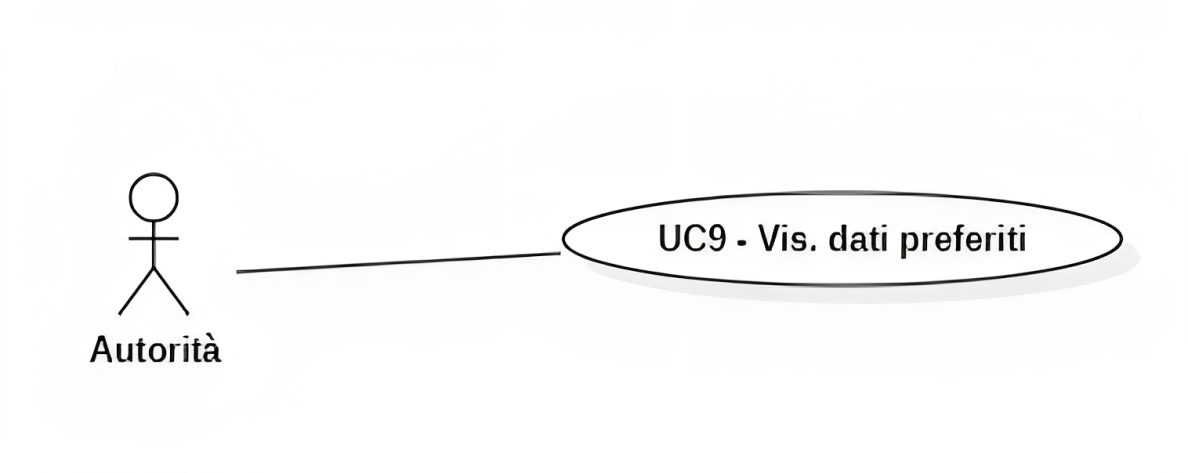
\includegraphics[width=0.9\textwidth]{../Images/uc9.png}
    \caption{UC9 - Visualizzazione dati preferiti}
    \label{fig:UC9}
\end{figure}
\subsubsection{UC9 - Visualizzazione dati preferiti}
\begin{itemize}
    \item \textbf{Attore principale:} Autorità locale;
    \item \textbf{Descrizione:} L’autorità locale seleziona la visulizzazione dei dati preferiti.
    \item \textbf{Scenario principale:}
          \begin{enumerate}
              \item L'utente accede alla piattaforma per la visualizzazione della dashboard sullo stato della città o di una cella(UC1) (UC1.1);
              \item L'utente sceglie di visualizzare la pagina dedicata alla visualizzazione dei dati preferiti.
          \end{enumerate}
    \item \textbf{Precondizioni:}
          \begin{itemize}
              \item  L'utente si trova nella pagina per la visualizzazione delle dashboard (UC1) (UC1.1);
          \end{itemize}
    \item \textbf{Postcondizioni:}
          \begin{itemize}
              \item  L'utente ha una visione dei dati dei sensori salvati come preferiti.
          \end{itemize}
    \item \textbf{User story associata:}
          \begin{itemize}
              \item Come di Autorità Locale, desidero visualizzare i dati dei sensori precedentemente salvati come preferiti sulla piattaforma, così da poter accedere rapidamente alle informazioni rilevanti.
          \end{itemize}
\end{itemize}

%---------------------------- UC10 ---------------------------------
\begin{figure}[H]
    \centering
    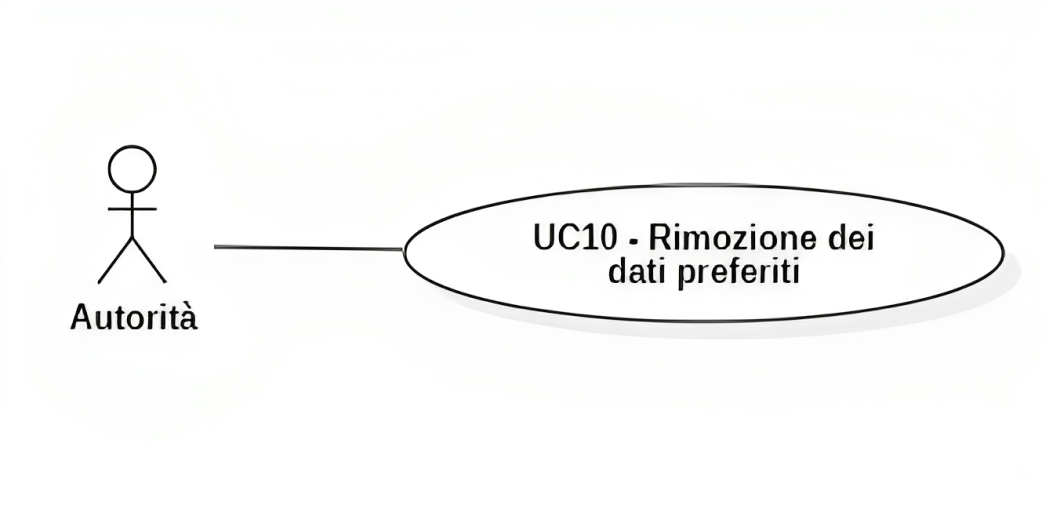
\includegraphics[width=0.9\textwidth]{../Images/uc10.png}
    \caption{UC10 - Rimozione dati preferiti}
    \label{fig:UC10}
\end{figure}
\subsubsection{UC10 - VISUALIZZAZIONE WIDGET SENSORI ISOLE ECOLOGICHE}
\begin{itemize}
    \item \textbf{Attore principale:} Autorità locale;
    \item \textbf{Precondizioni:}
        \begin{itemize}
            \item Almeno un sensore di rilevamento soglia delle isole ecologiche ha trasmesso dati al sistema;
            \item Il sistema ha caricato la visualizzazione della dashboard (UC1).
        \end{itemize}
    \item \textbf{Postcondizioni:}
        \begin{itemize}
            \item L'autorità locale visualizza un widget contenente le misurazioni relative ai sensori di rilevamento soglia delle isole ecologiche.
        \end{itemize}
    \item \textbf{Scenario principale:}
        \begin{enumerate}
            \item Il sistema carica i dati e imposta la visualizzazione del widget contenente le misurazioni relative ai sensori di rilevamento soglia delle isole ecologiche.
        \end{enumerate}
    \item \textbf{User story associata:} \\
        Come autorità locale, desidero visualizzare un widget per la visualizzazione delle misurazioni trasmesse dai sensori di rilevamento soglia delle isole ecologiche. Questo mi permetterà di analizzare in modo approfondito i dati relativi a quella tipologia di sensori, aiutandomi a prendere decisioni mirate per migliorare i servizi della città.
\end{itemize}

%---------------------------- UC ---------------------------------
\newcounter{rowcounter}
\setcounter{rowcounter}{1}
